\begin{figure}[t]
  \hspace{0.05\textwidth}%
  \begin{subfigure}[b]{\textwidth}
    \tikzstyle{legend-point}=[circle, inner sep=2pt]
    \definecolor{m-octree}{HTML}{966687}
    \definecolor{r-octree}{HTML}{837150}
    \definecolor{m-data}{HTML}{697b9c}
    \definecolor{r-data}{HTML}{568665}
    
    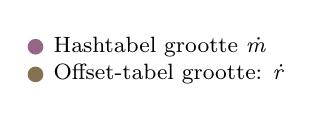
\begin{tikzpicture}
      \node (legend:1) at (0.1\textwidth,   0pt) [legend-point, fill={m-octree}, label=right:{\footnotesize Hashtabel grootte $\mathit{\dot{m}}$}] {};
      \node (legend:2) at (0.1\textwidth, -10pt) [legend-point, fill={r-octree}, label=right:{\footnotesize Offset-tabel grootte: $\mathit{\dot{r}}$}] {};
    \end{tikzpicture}
  \end{subfigure}\hfill\\
  \begin{adjustbox}{minipage=\textwidth, scale=0.55}
    \begin{subfigure}[b]{0.8\textwidth}
      \centering
      \def\svgwidth{\textwidth}
      \input{./img/raw/hs-layered-mem/layered_spaceship-indoor_1260_octree.pdf_tex}
      \caption{Spaceship Indoor - octreebeschrijving}
      \vspace{4pt}
      \label{fig:hs-layered-mem:indoor-octree}
    \end{subfigure}
  \end{adjustbox} %
  %
  \begin{adjustbox}{minipage=\textwidth, scale=0.55}
    \begin{subfigure}[b]{0.8\textwidth}
      \centering
      \def\svgwidth{\textwidth}
      \input{./img/raw/hs-layered-mem/layered_spaceship-indoor_1260_data.pdf_tex}
      \caption{Spaceship Indoor - lichtbeschrijving}
      \vspace{4pt}
      \label{fig:hs-layered-mem:indoor-data}
    \end{subfigure}
  \end{adjustbox} \\
  %
  \begin{adjustbox}{minipage=\textwidth, scale=0.55}
    \begin{subfigure}[b]{0.8\textwidth}
      \centering
      \def\svgwidth{\textwidth}
      \input{./img/raw/hs-layered-mem/layered_pipers-alley_1044_octree.pdf_tex}
      \caption{Piper's Alley - octreebeschrijving}
      \label{fig:hs-layered-mem:alley-octree}
    \end{subfigure}
  \end{adjustbox}
  %
  \begin{adjustbox}{minipage=\textwidth, scale=0.55}
    \begin{subfigure}[b]{0.8\textwidth}
      \centering
      \def\svgwidth{\textwidth}
      \input{./img/raw/hs-layered-mem/layered_pipers-alley_1044_data.pdf_tex}
      \caption{Piper's Alley - lichtbeschrijving}
      \label{fig:hs-layered-mem:alley-data}
    \end{subfigure}
  \end{adjustbox} \\
  %
  \begin{adjustbox}{minipage=\textwidth, scale=0.55}
    \begin{subfigure}[b]{0.8\textwidth}
      \centering
      \def\svgwidth{\textwidth}
      \input{./img/raw/hs-layered-mem/layered_ziggurat-city_1170_octree.pdf_tex}
      \caption{Ziggurat City - octreebeschrijving}
      \label{fig:hs-layered-mem:city-octree}
    \end{subfigure}
  \end{adjustbox} %
  %
  \begin{adjustbox}{minipage=\textwidth, scale=0.55}
    \begin{subfigure}[b]{0.8\textwidth}
      \centering
      \def\svgwidth{\textwidth}
      \input{./img/raw/hs-layered-mem/layered_ziggurat-city_1170_data.pdf_tex}
      \caption{Ziggurat city - lichtbeschrijving}
      \label{fig:hs-layered-mem:city-data}
    \end{subfigure}
  \end{adjustbox}
  \caption{\small Geheugen gebruik per laag van de Hashed Shading datastructuren als functie van de knoopgrootte.}
  \label{fig:hs-layered-mem}
\end{figure}

